\chapter{Einführung in Reactive Programming mit RxJava2}\label{rp_einfuehrung}
ReactiveX ist ein Open Source Projekt und vereint reaktive Bibliotheken für viele Sprachen und Frameworks unter einem Dach. Die Bibliotheken halten sich an den gleichen Aufbau und Benennung um eine gewisse Konsistenz zu schaffen. Die erste dieser Bibliotheken wurde unter Leitung von Erik Meijer bei Microsoft entwickelt und nennt sich Rx.NET, als Erweiterung zum .NET Framework von Microsoft. Das Kürzel \textit{Rx} steht für Reactive Extentions, also reaktive Erweiterungen. Folgend wurde von Ben Christensen und Jafar Husain als Entwickler bei Netflix die Erweiterung für Java geschrieben und auf GitHub veröffentlicht. Es folgten viele weitere Implementierungen für zum Beispiel Ruby, Python oder JavaScript. Die Bibliothek der Reactive Extensions ist sehr klein, bringt jedoch die nötigen Eigenschaften mit, um asynchrone und nicht blockierende Anwendungen zu entwickeln. ReaktiveX sagt über sich, dass die besten Ideen des Beobachtermusters, des Iteratormusters sowie der funktionalen Programmierung hinter ihrer Art der Implementierung stecken. Die teilweise schon in Java vorhandenen Klassen wie der Observer wurden überlagert und für ein reaktives Verhalten gerüstet. Aktuell wird RxJava als Version 1 und Version 2 entwickelt. In Version 2 wurden Änderungen vorgenommen um den Vorgaben der Asynchronität und der Verwendung des Back Pressures der Reactive Streams Initiative zu genügen. Da es sich nicht nur um eine Erweiterung sondern um eine Neuentwicklung parallel zu Version 1 handelt, sind im Moment beide Versionen im Entwicklungsstatus. RxJava2 wird in dieser Arbeit als Referenzbibliothek verwendet.\cite{rxgit}.\\ Der zentrale Baustein dieser Bibliothek ist die Observable-Klasse im Zusammenspiel mit dem Observer Interface. Ein Observable repräsentiert einen Data- beziehungsweise Eventstream. Es ist für das Push-Verfahren konzipiert (reaktiv), kann aber auch mit dem Pull-Verfahren verwendet werden (interaktiv) \cite{Nurkiewicz.2017}. Es folgt nun eine kurze Schilderung wie die wichtigsten Eigenschaften erreicht werden bevor die eigentliche Struktur, im Genauen eine Beschreibung der Basisklassen der Bibliothek, veranschaulicht wird. Diese Eigenschaften wurden vom bereits erwähnten Ben Christensen in Kapitel 1 innerhalb des Buches von Tomasz Nurkiewicz beschrieben \cite{Nurkiewicz.2017}. 
\section{Synchronität und Asynchronität}
Bei dem bisher gelesenen wird schnell klar, dass die Asynchronität ein essentieller Bestandteil sein muss. Jedoch ist das Observable standardmäßig synchron implementiert und ein asynchrones Verhalten muss explizit gefordert werden. Erfolgt eine Registrierung(Subscription) eines Observers an einem Observable, wird die Weitergabe der Elemente des Streams auf dem Thread des Observers ausgeführt. Ebenso finden die Bulk Operations, also Transformation, Modifikation und Komposition der Elemente oder Streams grundsätzlich synchron statt. Werden also Daten zum Beispiel aus einem Cache geladen und über den Stream zur Verfügung gestellt ist der Standardweg des synchronen Vorgehens vollkommen richtig um den Overhead der expliziten Asynchronität zu umgehen. Finden aber Abfragen, zum Beispiel über eine Netzwerkressource, statt, die unterschiedliche lange Latenzen aufweist, kann es notwendig sein, die Anfragen auf weiteren Threads auszuführen. Dies kann mittels eigens erstellter Threads, Threadpools oder Schedulers umgesetzt werden. Somit werden die Callback-Methoden des Observers von dem zusätzlichen erstellten Thread aufgerufen und der eigentliche Observer Thread wird nicht weiter blockiert.
\section{Parallelisierung und Nebenläufigkeit}
Parallelisierung und Nebenläufigkeit sind vor allem auf Systemebene zu betrachten. Nebenläufigkeit besagt, dass mehrere Tasks gleichzeitig ausgeführt werden können. Findet diese Bearbeitung auf physisch unterschiedlichen Kernen zur gleichen Zeit statt, spricht man von paralleler Ausführung. Ist jedoch nur ein Kern vorhanden oder Tasks werden trotz mehrerer Kerne auf nur einem ausgeführt, findet eine sequentielle Abarbeitung statt. Der Kernel des Systems bringt hierfür die Funktion des \textit{time-slicing} mit. Diese regelt, wann welcher Task Rechenzeit zugewiesen bekommt. Um dieses Verfahren in Verbindung mit den Observables zu bringen, gilt, dass ein Observable Stream immer serialisierbar und thread-safe sein muss. Die Callback-Methoden des Subscribers können also nie zeitgleich aufgerufen werden. Dieser Vertrag muss eingehalten werden, um die Funktionalität des Observables zu gewährleisten.
\section{Push und Pull}
Wird Pulling von Objekten einer Liste über das Iterable Interface durchgeführt, so wird im Gegenzug Pushing via Observable realisiert. Beide Schnittstellen bieten die gleiche Funktionalität, nur der Datenfluss findet in die entgegengesetzte Richtung statt. Durch diese Dualität können beide Vorgehen äquivalent verwendet werden. Will man ein weiteres Objekt einer Liste über den Iterator abfragen, wird die \textit{next()}-Methode aktiv aufgerufen und, wenn vorhanden, wird ein weiteres Objekt dem Verbraucher zurück gegeben. Hingegen wird bei der Verwendung von Observables die Daten des Streams mit der \textit{onNext()}-Methode des Verbrauchers gepusht. Wie die Tabelle \ref{tbl:vglIterObs} zeigt, gilt dies ebenso beim Auftreten eines Fehlers oder beim Erreichen des Endes der Datenquelle.
\begin{table}[]
	\centering
	\begin{tabular}{|c|c|lll}
		\cline{1-2}
		\cellcolor[HTML]{C0C0C0}Pull (Iterable) & \cellcolor[HTML]{C0C0C0}Push (Observable) &  &  &  \\ \cline{1-2}
		T next()                                & onNext(T)                                 &  &  &  \\ \cline{1-2}
		throws Exception                        & onError(Throwable)                        &  &  &  \\ \cline{1-2}
		returns                                 & onComplete()                             &  &  &  \\ \cline{1-2}
	\end{tabular}
	\caption{Vergleich zwischen Funktionalität der Iterable- und Observable-Schnittstelle.}
	\label{tbl:vglIterObs}
\end{table}
Die Verbindung zwischen Observable und Observer findet über ein Subscription statt. Damit werden die beiden zu einem Paar gebunden und die entsprechenden Methoden des Observers können nun von dem Stream angesprochen werden. Dies beschreibt auch noch eine weitere Eigenschaft. Ein Observable publiziert nur die Ereignisse wenn es jemanden gibt der diese Ereignisse auch anfordert. Dies wird auch als \textit{Lazy Initialization} bezeichnet. Somit wird das Arbeiten durch das Subscriben und nicht durch das Erstellen eines Observables angestoßen. Im Vergleich dazu kann ein Objekt vom Typ Future betrachtet werden. Wird ein Future erstellt beginnt die einmalige asynchrone Ausführung der Aufgabe. Das Resultat wird innerhalb des Futures zur Verfügung gestellt sobald die Aufgabe abgeschlossen ist. Ein mehrfaches Ausführen eines Futures ist nicht möglich, anders als beim Observable wo zu jeder Zeit ein weiterer Subscriber hinzu kommen kann. Durch dieses Verhalten wird die Wiederverwendbarkeit des Observables erreicht. 
\section{Observable}
Es wurde in den vorherigen Abschnitten schon einiges über das Observable-Objekt gesagt, doch zur Vervollständigung werden hier die Eigenschaften und Fähigkeiten zusammengefasst beschrieben. Es handelt sich hierbei um das Kernelement der RxJava Bibliothek.
\lstinputlisting[linerange={7-13}, float=hbt, caption={Beispiel Observable Initialisierung und Subscription}, label=lst:obsexample]{../SystemMonitor/examples/obs/ObservableExample.java}
Ein Ereignisstrom über einen Zeitraum wird von einem Observable repräsentiert. Dieser Ereignisstrom ist jedoch variabel. Weder muss die Anzahl der auftretenden Ereignisse bekannt sein, noch müssen diese in einem geregelten Intervall auftreten. Ebenso wenig muss der Zeitraum begrenzt sein, was bedeutet, dass es sich auch um unendliche Eventstreams handeln kann. Die Tabelle \ref{tbl:vglIterObs} zeigt die Methodenaufrufe, die eine Observable auslösen kann. Somit wird auch klar, dass nur drei Arten von Events auftreten können. Eine beliebige Anzahl von \textit{onNext(T)}-Methodenaufrufen mit dem Eventtyp T, das einmalige Event der Fertigstellung mit dem \textit{onComplete()}-Aufruf oder das Aufkommen eines Fehlers mit der \textit{onError(Throwable)}-Methode. Somit gilt: 
\begin{displaymath}
	OnNext*(OnComplete | OnError)?
\end{displaymath}
Daraus resultiert, dass entweder ein gewolltes Ende oder ein unvorhergesehener Fehler auftritt, aber niemals beides. Schaut man sich nun Listing \ref{lst:obsexample} an, sieht man den Ablauf. Ein Observable wird initialisiert, hier mit drei Elementen, also ein endlicher Stream. Durch das \textit{subscribe} wird anonym ein Subscriber erzeugt. Bei dem ersten Lambda-Ausdruck handelt es sich um die \textit{onNext()}-Methode. Weiter geht es mit \textit{onError()} und \textit{onComplete()}. Man sieht bei einem fehlerfreien Durchlauf die drei Elemente auf der Konsole und ebenso die Ausgabe für das Beenden des Streams. Würde ein Fehler auftreten, würde die Ausgabe der Elemente beendet werden und der Stacktrace würde ausgegeben werden, statt des \textit{finish}-Strings. Auch wurde schon ein wichtiger Punkt angeschnitten, nämlich, dass zu jeder Zeit ein neuer Subscriber hinzu kommen kann. Jeder Subscriber erhält einen separaten Observable Stream. Observables mit dieser Eigenschaft nennt man auch \textit{Cold Observable}.
\lstinputlisting[linerange={11-16}, float=hbt, caption={Beispiel Cold Observable}, label=lst:coldobs]{../SystemMonitor/examples/cold/ColdObs.java}
Wie hier in Listing \ref{lst:coldobs} zu sehen werden zwei Objekte des Observable-Streams erstellt. Es ist zu beachten, dass somit jeder Subscriber einen eigenen Timer bekommt. Will man nun aber die beiden Rechenoperationen immer auf den selben Wert durchführen, wird es auf diesem Wege nicht funktionieren. Somit muss es die Möglichkeit geben diese Informationen zu teilen.
\lstinputlisting[linerange={12-20}, float=hbt, caption={Beispiel Hot Observable}, label=lst:hotobs]{../SystemMonitor/examples/hot/HotObs.java}
Der Methodenaufruf \textit{publish()} ist hier der Schlüssel. In Listing \ref{lst:hotobs} sieht man diesen Aufruf nachdem das Intervall gestartet wird. Durch diesen Aufruf erhält man eine besondere Form des Observables, das \textit{ConnectableObservable}. Grundlegend hat sich am Aufbau des Observables nichts geändert, jedoch beginnt das Ausgeben der Daten nicht durch eine Subscription, sondern durch das Aufrufen der \textit{connect()}-Methode. Durch diese Eigenschaft wird das Observable zu einem sogenannten \textit{Hot Observable}. Schaltet sich nun ein Subscriber auf den Stream, beginnt er mit den Werten der zu diesem Zeitpunkt ausgegeben wird. Die schon vergangenen Events sind für den Subscriber nicht mehr zu erreichen. Es macht zum Beispiel Sinn, wenn eine Mausbewegung getrackt wird, da neue Subscriber nicht wissen müssen wo sich der Mauszeiger vorher befand, denn es ist nur wichtig wo sich der Zeiger aktuell befindet. Je nach Problemstellung ist das eine oder das andere von Vorteil. Ist es entscheidend eine konsistente und vollständige Abarbeitung von Events durchzuführen greift man auf Cold Observables zurück. Handelt es sich um einen Stream über den man keine konkrete Kontrolle hat, wie ein Stream für Ein- und Ausgabe, wird man meist Hot Observables verwenden. \\ Ein Punkt welcher das Observable nicht vollständig abdeckt, ist der Back Pressure. Es sind keine Möglichkeiten enthalten um aktiv auf Back Pressure reagieren zu können. Wie schon erwähnt ist seit Version 2 der RxJava Bibliothek eine Implementierung diese Möglichkeit nach Richtlinien der Reactive Stream Initiative vorhanden. Dies wurde in der Klasse \textit{Flowable} implementiert.
\section{Flowable}
Diese Klasse ist nach den Kriterien der Reactive Streams realisiert, was wiederum heißt, eine asynchrone Bearbeitung ohne blockender Back Pressure muss möglich sein. Durch die Implementierung \textit{org.reactivestreams.Publisher<T>} des Publisher Interfaces wird die Handhabung des Back Pressures ermöglicht und da auch die Funktionalität des Observables vorhanden ist, kann eine Bearbeitung asynchron stattfinden. In der offiziellen Dokumentation von RxJava2 wird beschrieben, wann es sich besser eignet auf Observables oder aber auf Flowables zu setzen \cite{rxdifference}. \underline{Wann sollte man Observables nutzen:}
\begin{itemize}
	\item Wenn im Datenfluss nicht mehr als 1000 Elemente auftreten, es somit als keine Chance für einen \textit{OutOfMemoryError} gibt.
	\item Wenn GUI Events behandelt werden. Diese können durch ihr unregelmäßiges Aufkommen schlecht gepuffert werden. Außerdem ist das Auftreten meist geringfügig. Elemente in der Auftrittshäufigkeit von maximal 1000 Hz sollten zu bewältigen sein.
	\item Wenn die Plattform keine Streams unterstützt, also die Java Version diese noch nicht bereit stellt. Grundsätzlich bringen Observables weniger Overhead mit sich.
\end{itemize} \newpage
\underline{Wann sollte man Flowables nutzen:}
\begin{itemize}
	\item Wenn mehrere Tausende Elemente generiert werden und die Möglichkeit vorhanden ist mit der Quelle zu kommunizieren, um bei fehlendem Back Pressure die Frequenz zu regeln.
	\item Beim Lesen von der Festplatte. Dies geschieht blockierend und mit dem Pull-Ansatz, was sich hervorragend eignet um die Elemente als Back Pressure zu puffern.
	\item Beim Lesen aus der Datenbank. Auch dieser Zugriff funktioniert mit dem Pull-Ansatz und blockiert. Also wieder von Vorteil mit einem Puffer zu arbeiten.
	\item Kommunikation über ein Netzwerk. Hierbei kann, sofern unterstützt, eine logische Menge an Elementen angefragt werden, welche im Puffer gesichert wird. Die gepufferten Elemente können nun stetig abgearbeitet werden.
	\item Weiter blockierende auf Pull-basierenden Datenquellen deren API eventuell in Zukunft auch auf ein reaktives Verhalten umgestellt werden. Hier liegt der Vorteil in der Reactive Streams Konvention die voraussichtlich auch in Zukunft verwendet wird.
\end{itemize}
\lstinputlisting[linerange={10-17, 19-33, 49-49}, float=hbt, caption={Beispiel Flowable mit BackPressureBuffer}, label=lst:flowexample]{../SystemMonitor/examples/flow/FlowExample.java}
Jedes Observable und Flowable Objekt besitzt einen Puffer um nicht verarbeitete 
Daten zwischen zu speichern. Diese Größe beträgt bei Flowables standardmäßig 128 
Objekte, kann jedoch geändert werden. Bei Observables ist dieser Puffer 
dynamisch und kann wenn nötig den kompletten Speicher beanspruchen. Betrachtet 
man das Listing \ref{lst:flowexample} sieht man den Aufruf der 
\textit{onBackpressureBuffer()}-Methode. Diese Methode bietet ein 
Observable-Objekt nicht. Es handelt sich um eine Implementierung des 
Publisher-Interfaces. Hiermit kann direkt eine Puffergröße für jedes Flowable 
festgelegt werden. Kann nun ein Subscriber also nur eine gewisse Anzahl von 
Elementen verarbeiten, kann über den bereits erwähnten Feedback-Kanal des 
Flowable informiert werden, die Objekte wenn möglich langsamer auszugeben. Die 
Verzögerung wird durch den zusätzlichen Puffer der 
\textit{onBackpressureBuffer()}-Methode ermöglicht. Die funktionsweise dieses 
Buffers lässt sich mit Abbildung \ref{pic:bbbuffer} aus der 
RxJava2 JavaDoc nachvollziehen. In diesem Beispiel wäre dieser Aufruf zwar 
nicht notwendig, doch zur Veranschaulichung wurde er hinzugefügt. Da auch die 
Anzahl der Elemente bekannt ist, kann der Puffer natürlich genau auf die Anzahl 
der Elemente festgelegt werden.
Um nun die Verwendung des Feedback-Kanals noch zu betrachten, wurde das 
Beispiel um einen \textit{DefaultSubscriber} erweitert.
\begin{figure}[hbt]
	\centering
	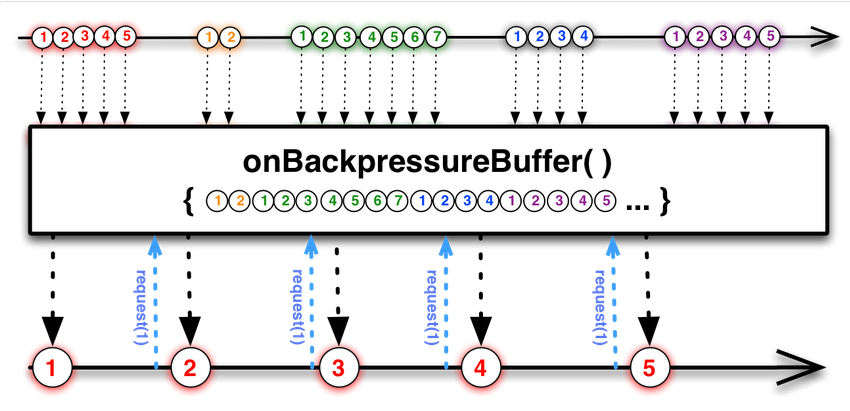
\includegraphics[width=1\textwidth]{Abb/backpressurebuffer}
	\caption{Funktionsweise BackPressureBuffer.}
	\label{pic:bbbuffer}
\end{figure}
Durch den Aufruf der \textit{onStart()}-Methode wird direkt zu Beginn der Subscription durch den \textit{request(1)} Aufruf die verträgliche Menge des Subscribers weiter gegeben. Ebenso findet diese Anfrage auch beim Aufruf jedes \textit{onNext()} Callbacks statt. Durch diesen Aufruf erfährt das Flowable, dass immer nur ein Element an den Subscriber ausgegben werden soll. Die beiden weiteren Elemente würden nun im BackPressureBuffer unterkommen und bei weiteren Anfragen zur Verfügung gestellt werden. Wie schon erwähnt ist dies in diesem kurzen Beispiel jedoch nicht nötig und dient nur zur Erklärung der Funktionsweise.
\section{Single}
Wo Observables oder Flowables eine Menge zwischen Null und unendlich vielen Elementen ausgeben, steht Single, wie der Name schon sagt, dafür, dass immer nur einmal auf ein einziges Event reagiert werden kann. Somit sind auch die drei bekannten Methoden zur Datenausgabe hier nicht notwendig. Stattdessen sind nur zwei Methoden vorhanden, \textit{onSuccess()} und \textit{onError()}. Auch hier gilt, dass immer nur eine der Methoden aufgerufen werden kann. Also eine erfolgreiche Datenausgabe oder eine fehlerbehaftete. Anschließend werden die Subscriptions gelöst und das Single wird beendet. Auch hier sind wieder eine Reihe von Bulk Operations möglich. 
\lstinputlisting[linerange={7-14}, float=hbt, caption={Beispiel eines Singles}, label=lst:singleexample]{../SystemMonitor/examples/single/SingleExample.java}
In Listing \ref{lst:singleexample} sieht man die Verwendung eines Single-Objekts. Es kann nur mit einem Objekt erstellt werden, die Bearbeitung dieses Elements findet wieder mit einer Auswahl an bekannten Operationen statt. In der \textit{subscribe()}-Methode sieht man die zwei Lambda-Ausdrücke die wieder die möglichen Methodenaufrufe, also bei Erfolg oder Fehlerfall, repräsentieren. Ein Beispiel für die Verwendung von Single findet sich zum Beispiel bei einer HTTP-GET Anfrage. Man möchte ein Objekt abrufen, und sobald es angekommen ist, soll es verwendet werden. Die Verwendung eines Single-Objekts ist hier plausibel, da für jede Anfrage immer ein Objekt zurück geliefert wird. Geht die Anfrage raus muss nicht gewartet werden und sobald das Ergebnis eingetroffen ist, wird die \textit{onSuccess()}-Methode aufgerufen oder eben im Fehlerfall die \textit{onError()}-Methode. 
\section{Subject}
Als Subject versteht man ein Objekt, dass sowohl als Observable und ebenso als Observer fungiert. Es kann an ein Observable subscriben, diese Daten verarbeiten und seinen eigenen Subscribern weiterleiten. 
\lstinputlisting[linerange={7-14}, float=hbt, caption={Beispielverwendung eines Subjects}, label=lst:subjectexample]{../SystemMonitor/examples/subject/SubjectExample.java}
Um das Vorgehen bei Verwendung eines Subject zu veranschaulichen betrachtet man 
Listing \ref{lst:subjectexample}. Es wird wieder das schon bekannte 
Observable-Objekt erstellt, hinzu kommt ein Subject, hier speziell eines vom Typ 
PublicSubject. Dieses Subject bekommt eine Subscription in welcher alle 
String-Werte in Großbuchstaben umgewandelt und anschließend auf der Konsole 
geschrieben werden. Wenn nun das Subject selbst an dem vorhandenen Observable 
subscribed, werden die von diesem ausgegebenen Werte gemapped und an die 
Subscriber des Subject weitergegeben. Zusätzlich zum PublicSubject stehen noch 
weitere Arten zur Verwendung bereit:
\begin{itemize}
	\item \underline{AsyncSubject:} Ein AsyncSubject gibt seinen Subscribern nur den letzte Wert der Quelle weiter und das auch nur falls das Quell-Observable beendet wurde. Endet es durch einen Fehler wird die Fehlermeldung direkt an die Subscriber des Subjects weiter gereicht.
	\item \underline{BehaviorSubject:} Ein BehaviorSubject beginnt sobald es einen Subscriber verzeichnen kann mit der Übermittlung des letzten Wertes der Quelle oder mit einem Standardwert falls von der Quelle noch nichts ausgegeben wurde. Anschließend werden alle weiteren Werte weitergegeben. Auch hier wird bei Auftreten eines Fehlers die Meldung direkt durchgereicht.
	\item \underline{PublishSubject:} Ein PublishSubject überträgt genau die Werte, die von seiner Quelle in dem Zeitraum, in welchem auch eine Subscription vorliegt, ausgegeben wurden. Alles vorherige wird nicht übermittelt. Somit liegt ein Verhalten eines Hot-Observables vor.
	\item \underline{ReplaySubject:} Ein ReplaySubject überträgt an jeden Subscriber alle Werte, die jemals von seiner Quelle ausgegeben wurden. Dieses Vorgehen bedarf eines Puffers, was bei fehlerhaften Verwendung zu einem BackPressure-Fehlverhalten führen kann. 
\end{itemize}
Auch hier wurde auf Grund der Konformität zur Reactive Streams Initiative eine weitere Klasse implementiert, welche die Möglichkeit bietet, aktiv auf Back Pressure zu reagieren. Die Processor-Klasse.
\section{Processor}
Was das Flowable für das Observable ist, stellt der Processor für das Subject dar. Eine Implementierung um den Anforderungen der Reactive Streams gerecht zu werden. Die Kompatibilität und das Handling des Back Pressures stehen auch hier wieder im Vordergrund. Die vier Ausprägungen des Subject sind auch bei der Processor-Klasse wiederzufinden. Zusätzlich wurde noch der \textit{UnicastProcessor} implementiert. Hier wird nur genau ein Subscriber zugelassen über die komplette Existenz des Processor-Objekts. Wenn versucht wird dagegen zu verstoßen wird eine \textit{IllegalStateException} geworfen.
\lstinputlisting[linerange={7-15}, float=hbt, caption={Beispielverwendung eines Processors}, label=lst:processorexample]{../SystemMonitor/examples/processor/ProcessorExample.java}
In Listing \ref{lst:processorexample} ist ein einfaches Beispiel zu finden. Eine Ähnlichkeit zur Subject-Klasse ist erkennbar. Jedoch werden hier die Flowables verwendet, und das Back Pressure kann aktiv kontrolliert werden. Ist also bekannt das Schnittstellen nach den Richtlinien der Reactive Streams Initiative entwickelt wurden, ist es lohnenswert auf die Verwendung von Flowables und Processors zu setzen um auf einfachem Wege eine Kompatibilität zu ermöglichen.
\section{Schedulers}
Im Abschnitt zu Parallelisierung und Nebenläufigkeit wurde schon gesagt, dass jedes Observable-Objekt serialisierbar und thread-safe sein muss. Dadurch ergibt sich die Möglichkeit, Observables oder einzelne Bulk Operations auf unterschiedlichen Threads auszuführen. RxJava bringt hierfür einige Scheduler mit die unterschiedliche Arten von Threads oder Threadpools mitbringen, um Multithreading zu ermöglichen. Um zum Beispiel eine Berechnung auf einem anderen Thread auszuführen, bringt die Observable-Klasse zwei Methoden mit: \textit{subscribeOn()} und \textit{observeOn()}. Beide Funktionen nehmen einen Scheduler als Parameter entgegen, jedoch unterscheiden sie sich in ihrer Funktionsweise. 
\begin{itemize}
\item \underline{subscribeOn:} Wird diese Funktion aufgerufen wird jedes Element des Observable vollständig auf den vom Scheduler bereit gestellten Thread bearbeitet. Finden mehrere Aufrufe statt, wird immer nur der erste Aufruf durchgeführt, da die Ausführung des Observable durch die Thread-Sicherheit immer nur auf einem Thread stattfindet. 
\item \underline{observeOn:} Hier wird nicht der Observable Stream an sich betrachtet, sondern die einzelnen Elemente. Somit ist es möglich, dass Operationen und Subscriptions jedes Mal auf einem neuen Thread stattfinden können. Dies heißt wiederum, dass jeder Aufruf von \textit{observerOn} dazu führt, dass die folgenden Operationen auf dem neuen Thread ausgeführt werden.
\end{itemize}
\lstinputlisting[linerange={11-11, 17-19}, float=hbt, caption={Beispiele für Scheduling mit zwei subscribeOn-Aufrufen}, label=lst:subscribeon]{../SystemMonitor/examples/scheduling/SchedulerExample.java}
Listing \ref{lst:subscribeon} zeigt ein Observable welches eine Operation, eine Subscription und zwei \textit{subscribeOn}-Methodenaufrufe beinhaltet. In diesem Beispiel wird alles auf einem Thread ausgeführt. Dieser Thread wird von dem ersten auftretenden \textit{Schedulers.newThread()} erstellt und jeder weitere Aufruf wird ignoriert, da das komplette Observable nur auf einen Thread ausgeführt werden kann. Betrachtet man nun das Listing \ref{lst:observeon}, erkennt man die gleiche Struktur, jedoch wird in diesem Fall die \textit{observeOn}-Methode zweimal verwendet. Wie beschrieben wird hier jeder einzelne Bestandteil des Observables als einzelner Task behandelt und kann somit immer auf einem neuen Thread ausgeführt werden. Hier wird in beiden Methodenaufrufen ein eigener Thread erzeugt. Zur Veranschaulichung betrachtet man Tabelle \ref{schedulertable}. Die erste Spalte zeigt den Programmfluss des Listings \ref{lst:subscribeon}. Das Observable wird auf einem Thread immer pro Element durchlaufen. Im Vergleich dazu kann man in der zweiten Spalte den Programmfluss von Listing \ref{lst:observeon} sehen. Auf dem ersten Thread findet zuerst die Operation für das mapping von jedem Element statt und auf dem zweiten Thread die danach folgende Operation, in diesem Fall die Subscription.
\begin{table}[]
	\centering
	\begin{tabular}{|c|l|}
		\hline
		\rowcolor[HTML]{C0C0C0} 
		subscribeOn                                           & \multicolumn{1}{c|}{\cellcolor[HTML]{C0C0C0}observeOn} \\ \hline
		mapping: RxNewThreadScheduler-1                       & mapping: RxNewThreadScheduler-1 \\ \hline
		java: RxNewThreadScheduler-1						  & mapping: RxNewThreadScheduler-1 \\ \hline
		mapping: RxNewThreadScheduler-1 					  & mapping: RxNewThreadScheduler-1 \\ \hline
		kotlin: RxNewThreadScheduler-1  					  & java: RxNewThreadScheduler-2    \\ \hline
		mapping: RxNewThreadScheduler-1                       & kotlin: RxNewThreadScheduler-2  \\ \hline
		scala: RxNewThreadScheduler-1                         & scala: RxNewThreadScheduler-2   \\ \hline
	\end{tabular}
	\caption{Ablauf der Threads bei Verwendung von subscribeOn und observeOn}
\label{schedulertable}
\end{table}
Somit muss je nach Vorhaben und Anforderung die passende Art von Scheduling betrieben werden. 
\lstinputlisting[linerange={11-11, 31-33}, float=hbt, caption={Beispiele für Scheduling mit zwei observeOn-Aufrufen}, label=lst:observeon]{../SystemMonitor/examples/scheduling/SchedulerExample.java}

\section{Operationen}
Es wurde schon einiges über die auf Observable anwendbaren Bulk-Operations geschrieben und in manchen Listings auch angewandt, jedoch noch nicht im einzelnen geschildert wie der genaue Ablauf einer solchen Operation stattfindet. Um die ganze Mechanik besser zu verstehen, werden folgend vier der gängigen Operationen veranschaulicht. Hierzu werden sogenannte Marble-Diagramme verwendet. Die oberer Linie stellt immer ein Observable-Stream in zeitlichem Ablauf dar, also ähnlich einem Zeitstrahl. Jedes Element, dargestellt durch die farblichen \textit{Marbles}, wird durch die mittlere Operation geführt und auf das ausgehende Observable, am unteren Ende des Bildes ausgegeben.
\subsection{Operation filter()}
\begin{figure}[hbt]
	\centering
	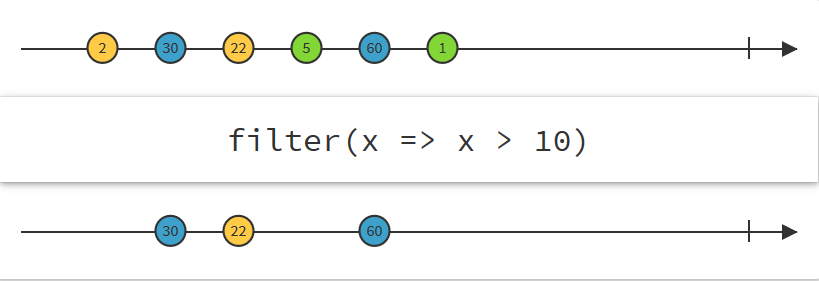
\includegraphics[width=1\textwidth]{Abb/filter}
	\caption{Datenfluss Filter-Operation}
	\label{pic:filter}
\end{figure}
\lstinputlisting[linerange={13-22}, float=hbt, caption={Beispiel Filter Operation}, label=lst:filterop]{../SystemMonitor/examples/operators/Ops.java}
Wie sich aus dem Namen schließen lässt, handelt es sich hierbei um eine Operation die jedes Element auf Kriterien überprüft, und sofern das Element gültig ist, wird es weitergeben. Verwendet wir hier der von RxJava mitgebrachte Datentyp \textit{Predicate}. Er beinhaltet eine Methode \textit{test()} zur Implementierung, welche ein \textit{boolean} zurück liefert. Somit ist es möglich einfache aber auch komplexere Überprüfungen innerhalb der Filter-Operation auszuführen. Im Bild \ref{pic:filter} sieht man eine Filterung nach dem Kriterium, dass nur jedes Element, das ein Wert größer 10 repräsentiert, ausgegeben wird. Da jedes Element sequentiell überprüft wird, erhält das untere Observable immer genau dann ein Element, wenn es auch zu diesem Zeitpunkt die Prüfung passiert hat. In Java-Code sieht das ganze dann aus wie in Listing \ref{lst:filterop}. Innerhalb des Predicate wird die \textit{test()}-Methode implementiert und die Prüfung, ob der Wert größer 10 ist, durchgeführt. 
Parametrisiert wird das Predicate auf den Wert Integer, da nur ein Datentyp übergeben wird, Resultat is immer Datentyp boolean. Das Predicate kann natürlich auch inline als Lambda oder anonym deklariert werden.
\subsection{Operation map()}
Die Map-Operation gilt als Transformationsoperation. Ihre Aufgabe ist es, jeden auftretenden Wert auf einen Funktionswert abzubilden und das Resultat auszugeben. In Abbildung \ref{pic:map} sieht man auf dem ursprünglichen Observable drei auftretenden Elemente. Jedes dieser Elemente wird mit 10 multipliziert und danach an das resultierenden Observable ausgegeben. 
\begin{figure}[hbt]
	\centering
	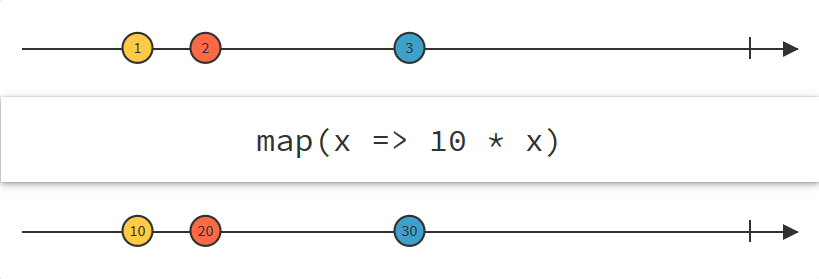
\includegraphics[width=1\textwidth]{Abb/map}
	\caption{Datenfluss Map-Operation}
	\label{pic:map}
\end{figure}
\lstinputlisting[linerange={25-26}, float=hbt, caption={Beispiel Map Operation}, label=lst:mapop]{../SystemMonitor/examples/operators/Ops.java} 
Innerhalb des Programmcodes wird es wie erwartet als Lambda-Ausdruck dargestellt. Das mapping bildet $x -> x \cdot 10$ ab.
\subsection{Operation merge()}
Merge repräsentiert eine Observable-Komposition. Es handelt sich hierbei um eine recht einfache Variante, denn es werden lediglich alle Elemente aus mindestens zwei Observables in einen Observable-Stream zusammengefasst. 
\begin{figure}[hbt]
	\centering
	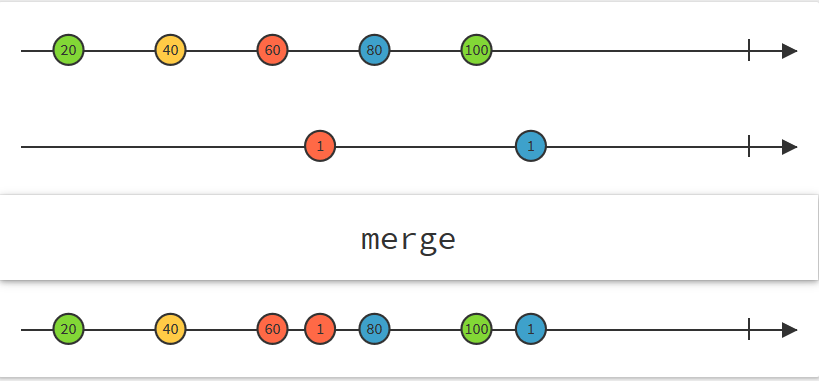
\includegraphics[width=1\textwidth]{Abb/merge}
	\caption{Datenfluss Merge-Operation}
	\label{pic:merge}
\end{figure}
Betrachtet man auch hier die passende Abbildung \ref{pic:merge} wird deutlich, wie die Komposition stattfindet. Zu jedem Zeitpunkt zu welchem eines der Observables ein Element ausgibt, wird es an das zusammengeführte Observable weitergegeben. Somit wird die Reihenfolge der Elemente rein von dem Faktor Zeit bestimmt.
\lstinputlisting[linerange={34-36}, float=hbt, caption={Beispiel Merge Operation}, label=lst:mergeop]{../SystemMonitor/examples/operators/Ops.java} 
Im Listing \ref{lst:mergeop} ist die entsprechende Implementierung zu sehen. Eines der Observables beinhaltet die Werte in zwanziger Schritten, das weitere produziert jede Nanosekunde ein Element. Das Mapping muss stattfinden, da immer nur Elemente eines Datentyps in einem Observable zusammengeführt werden können. Wie vorab schon erwähnt, kann die Unendlichkeit bei der Komposition von Streams zu Problemen hinsichtlich der Verwertbarkeit des Observerables und der Performanz einer Anwendung führen.
\subsection{Operation zip()}
Bei dem \textit{zip}-Operator handelt es sich ebenfalls um eine Komposition von Observables. Wie die Funktionsweise eines Reißverschlusses werden die Elemente miteinander verbunden. Abbildung \ref{pic:zipop} erläutert diese Weise genauer. Die Elemente der beiden Observables können unterschiedlichen Typs sein und können zu unterschiedlichen Zeitpunkten ausgegeben werden. Zip geht nun so vor, dass ab dem Moment, ab welchem mehrere Observables zusammen gelegt werden, immer die nächsten Elemente miteinander verknüpft werden und als Resultat ein neuer beziehungsweise anderen Datentyp entstehen kann.
\begin{figure}[hbt]
	\centering
	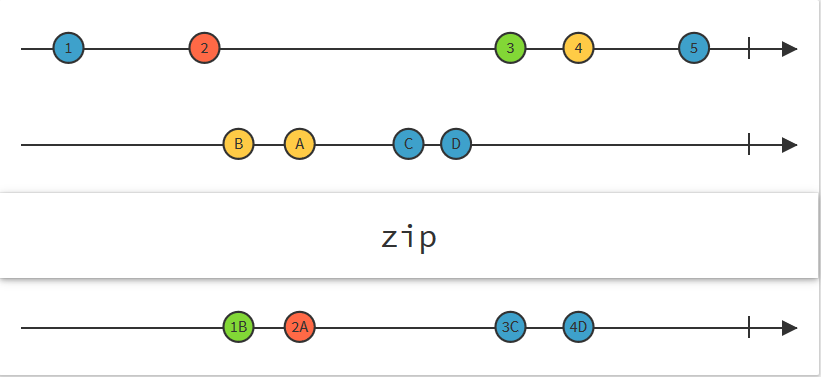
\includegraphics[width=1\textwidth]{Abb/zip}
	\caption{Datenfluss Zip-Operation}
	\label{pic:zipop}
\end{figure}
\lstinputlisting[linerange={29-31}, float=hbt, caption={Beispiel Zip Operation}, label=lst:zipop]{../SystemMonitor/examples/operators/Ops.java} 
Um es sich wieder von Entwicklungsseite zu veranschaulichen, ist in Listing \ref{lst:zipop} ein kurzes Beispiel dargestellt. Wie in der Abbildung werden einmal Zahlen, einmal Buchstaben als Observables repräsentiert und mit dem Zip-Operator verknüpft. Zip muss immer wissen wie die Objekte verbunden werden sollen. Hierzu wird eine entsprechende Funktion implementiert. Hier ist wieder die Verwendung von Lambdas möglich, wie es auch im Listing \ref{lst:zipop} stattfindet oder es muss eine explizite Funktion definiert werden, als Methode oder anonym. 